\section{Experiment Details}
\label{appendix:experiment_details}

\subsection{Rollout Results}
\label{appendix:rollout_results}

Table~\ref{tab:all_run_model_statistics} reports all 19 LLM rollouts: six models under ReAct, Reflection, and Plan-and-Act, and GPT-5.5 under ReAct only. All LLM rollouts use the \texttt{hard\_v2} configuration with environment seed 42; each model is run once under each of its evaluated scaffolds. Survival days follow the bankruptcy rule shared with the references, which stops a rollout after five consecutive \texttt{end\_today} closes with negative funds. Bold rows mark the rollout of each model with the longest survival, with final net worth and sales as tie-breakers; Appendix~\ref{appendix:stage_metrics} analyzes these seven rollouts in detail. Table~\ref{tab:framework_win_counts} counts, for the six models evaluated under all three scaffolds, how often each scaffold gives a model's best value. These are descriptive comparisons across three fixed scaffolds, not uncertainty estimates, and they do not causally separate base-model and scaffold effects.

\begin{table*}[t]
\centering
\footnotesize
\setlength{\tabcolsep}{2.5pt}
\renewcommand{\arraystretch}{1.06}
\resizebox{\textwidth}{!}{%
\begin{tabular}{llrrrrrr}
\toprule
Model & Scaffold & Days $\uparrow$ & Net worth $\uparrow$ & Sales $\uparrow$ & Return $\downarrow$ & Expired $\downarrow$ & Stockout-day rate $\downarrow$ \\
\midrule
\textbf{DeepSeek-V4-Pro} & \textbf{Plan-and-Act} & \textbf{180} & \textbf{10,120.90} & \textbf{164,417} & \textbf{0.0858} & \textbf{0.0144} & \textbf{0.6444} \\
DeepSeek-V4-Pro & ReAct & 144 & -1,554.47 & 134,931 & 0.0968 & 0.0573 & 0.5556 \\
DeepSeek-V4-Pro & Reflection & 94 & -1,792.13 & 33,593 & 0.0980 & 0.0452 & 0.7766 \\
GLM-5.1 & Plan-and-Act & 56 & -2,824.78 & 739 & 0.0338 & 0.0000 & 0.1964 \\
\textbf{GLM-5.1} & \textbf{ReAct} & \textbf{60} & \textbf{-2,134.36} & \textbf{7,016} & \textbf{0.1347} & \textbf{0.0297} & \textbf{0.2333} \\
GLM-5.1 & Reflection & 49 & 4,619.76 & 6,770 & 0.1145 & 0.0086 & 0.4694 \\
\textbf{GPT-5.5} & \textbf{ReAct} & \textbf{180} & \textbf{24,350.98} & \textbf{136,405} & \textbf{0.0646} & \textbf{0.0113} & \textbf{0.7611} \\
Grok-4.3 & Plan-and-Act & 12 & 22,989.16 & 372 & 0.0538 & 0.0000 & 0.4167 \\
\textbf{Grok-4.3} & \textbf{ReAct} & \textbf{58} & \textbf{828.40} & \textbf{11,305} & \textbf{0.1028} & \textbf{0.0577} & \textbf{0.4138} \\
Grok-4.3 & Reflection & 51 & 787.67 & 20,907 & 0.1286 & 0.1735 & 0.3529 \\
Kimi-K2.6 & Plan-and-Act & 89 & -1,996.52 & 48,955 & 0.0911 & 0.0016 & 0.6517 \\
\textbf{Kimi-K2.6} & \textbf{ReAct} & \textbf{130} & \textbf{792.19} & \textbf{86,214} & \textbf{0.1226} & \textbf{0.0411} & \textbf{0.4769} \\
Kimi-K2.6 & Reflection & 66 & 5,902.33 & 30,783 & 0.1121 & 0.0002 & 0.4697 \\
\textbf{MiniMax-M2.5} & \textbf{Plan-and-Act} & \textbf{73} & \textbf{-397.95} & \textbf{23,521} & \textbf{0.1077} & \textbf{0.0049} & \textbf{0.7123} \\
MiniMax-M2.5 & ReAct & 61 & 1,788.24 & 22,384 & 0.1041 & 0.0028 & 0.8197 \\
MiniMax-M2.5 & Reflection & 56 & 416.97 & 16,819 & 0.1041 & 0.0085 & 0.6607 \\
Qwen3.5-397B-A17B & Plan-and-Act & 50 & 3,820.59 & 30,074 & 0.1170 & 0.1055 & 0.5800 \\
Qwen3.5-397B-A17B & ReAct & 50 & 6,125.56 & 32,874 & 0.0968 & 0.0345 & 0.6800 \\
\textbf{Qwen3.5-397B-A17B} & \textbf{Reflection} & \textbf{71} & \textbf{1,183.17} & \textbf{35,622} & \textbf{0.1047} & \textbf{0.0655} & \textbf{0.6761} \\
\bottomrule
\end{tabular}
}
\caption{Complete outcome matrix for all 19 available LLM rollouts. Each row is one model--scaffold cell with a single rollout. \textbf{Bold} rows mark each model's longest-surviving rollout (ties broken by final net worth, then sales), analyzed in Figure~\ref{fig:failure_diagnostics}.}
\label{tab:all_run_model_statistics}
\vspace{-2mm}
\end{table*}

\begin{table}[t]
\centering
\footnotesize
\setlength{\tabcolsep}{2.5pt}
\renewcommand{\arraystretch}{1.06}
\resizebox{\columnwidth}{!}{%
\begin{tabular}{lrrrr}
\toprule
Metric & ReAct & Reflection & Plan-and-Act & Ties \\
\midrule
Survival days & 3 & 1 & 2 & 0 \\
Final net worth & 2 & 2 & 2 & 0 \\
Sales & 2 & 2 & 2 & 0 \\
Return ratio & 1 & 1 & 4 & 0 \\
Expired ratio & 2 & 1 & 3 & 0 \\
Stockout-day rate & 1 & 3 & 2 & 0 \\
\bottomrule
\end{tabular}
}
\caption{Scaffold win counts over the six models evaluated under all three scaffolds. Lower-is-better metrics are ranked in their preferred direction.}
\label{tab:framework_win_counts}
\vspace{-2mm}
\end{table}


\subsection{Four-Stage Diagnostic Metrics}
\label{appendix:stage_metrics}

\begin{figure*}[t!]
    \centering

    \begin{minipage}{0.48\textwidth}
        \centering
        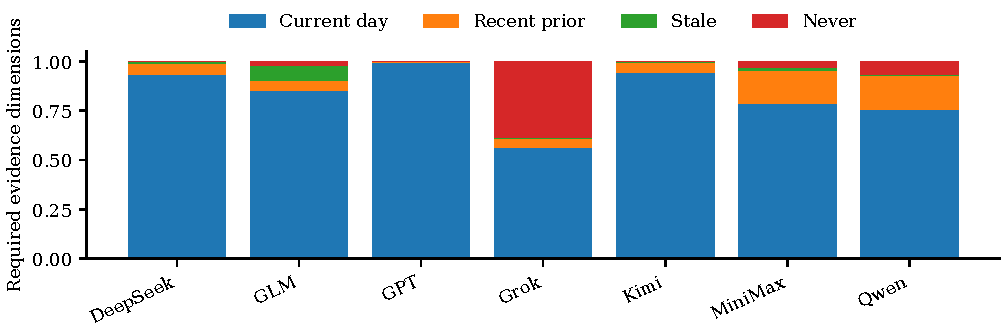
\includegraphics[width=0.99\linewidth]{figures/diagnostics_v2_stage2_evidence.pdf}
        \vspace{0.1em}
        \centerline{\small \textbf{(a) Trace evidence freshness}}
    \end{minipage}
    \hfill
    \begin{minipage}{0.48\textwidth}
        \centering
        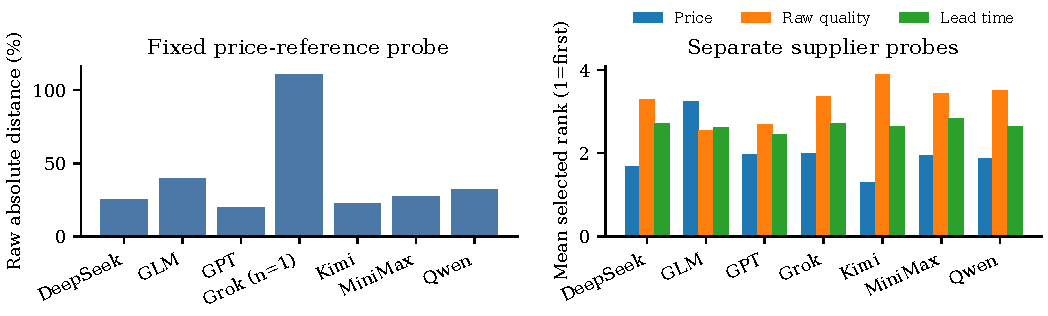
\includegraphics[width=0.99\linewidth]{figures/diagnostics_v2_stage3_action.pdf}
        \vspace{0.1em}
        \centerline{\small \textbf{(b) Independent action probes}}
    \end{minipage}

    \vspace{1.15em}

    \begin{minipage}{0.48\textwidth}
        \centering
        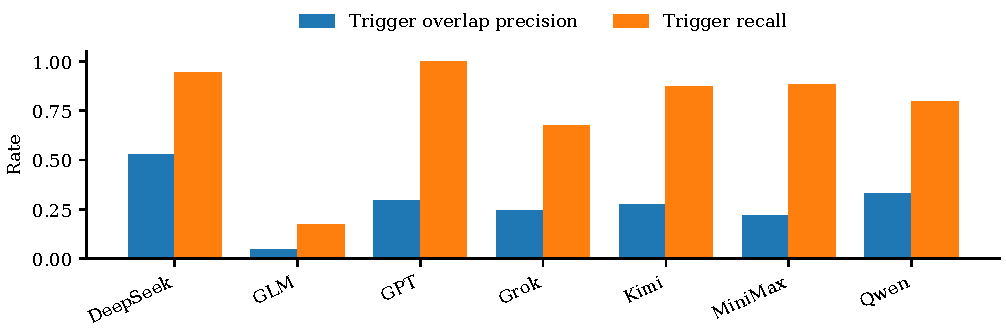
\includegraphics[width=0.99\linewidth]{figures/diagnostics_v2_stage1_attention.pdf}
        \vspace{0.1em}
        \centerline{\small \textbf{(c) Trigger-conditioned attention}}
    \end{minipage}
    \hfill
    \begin{minipage}{0.48\textwidth}
        \centering
        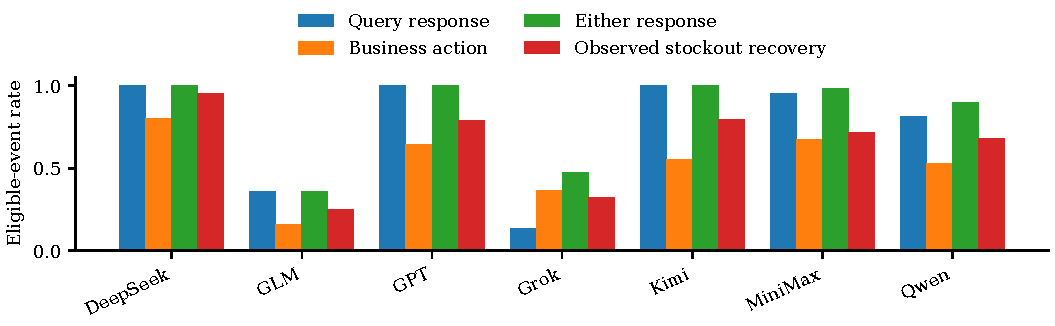
\includegraphics[width=0.99\linewidth]{figures/diagnostics_v2_stage4_response.pdf}
        \vspace{0.1em}
        \centerline{\small \textbf{(d) Event-conditioned response and recovery}}
    \end{minipage}

    \caption{Detailed per-stage diagnostics (diagnostics v2) for one survival-first rollout per LLM (longest survival, then final net worth and sales). Panel (a) partitions required evidence dimensions into current-day, recent-prior within a predeclared TTL, stale, and never observed states. Panel (b) reports an unnormalized fixed-reference price distance and three separate supplier ranks; Grok's price distance has only one valid reference action. Panel (c) measures overlap between attention and adverse events observable before the decision. Panel (d) separates successful query response, executed business action, either response, and conservative observed stockout recovery. The axes are descriptive probes with different interpretations, not a common utility scale.}
    \label{fig:failure_diagnostics}
\end{figure*}

This section defines the four headline scores in Figure~\ref{fig:four_stage_scores} and the detailed per-stage breakdowns in Figure~\ref{fig:failure_diagnostics}. All quantities are computed from successfully completed days; calls in an incomplete terminal day are excluded. A tool query counts only when it succeeds and returns material evidence for the requested product. The metrics are descriptive probes rather than reward terms or a global system ranking. Let $T$ be the number of completed days.

\paragraph{Headline scores.}
\textbf{Stage 1: Product Monitoring.} Let $\mathcal{Y}_{t}$ be the products with positive sales on day $t$ and $\mathcal{Q}_t$ the products receiving a successful product-specific query on day $t$; store-wide inventory or order listings do not count. Then
\begin{equation}
S_1=\frac{\sum_{t=2}^{T}|\mathcal{Y}_{t-1}\cap\mathcal{Q}_t|}{\sum_{t=2}^{T}|\mathcal{Y}_{t-1}|}.
\end{equation}
\textbf{Stage 2: Evidence Collection.} $S_2=\mathrm{FullFresh}$, the share of executed action--product events whose required evidence dimensions are all current-day or recent-prior (defined below).

\textbf{Stage 3: Decision-Making.} $S_3$ is the share of successful order lines whose chosen supplier has the highest raw simulator quality among the product's five suppliers. Raw quality is evaluator-only hidden state.

\textbf{Stage 4: Anomaly Response.} Let $\mathcal{E}$ contain the stockout and expiration events, identified by completed day $t_e$, event type, and product, with $t_e+3\leq T$; events with $t_e+3>T$ are right-censored. Let $r(e)=1$ if an executed order or price change on the same product occurs on a day in $\{t_e+1,t_e+2,t_e+3\}$. Then
\begin{equation}
S_4=\frac{\sum_{e\in\mathcal{E}}r(e)}{|\mathcal{E}|}.
\end{equation}
Per-model LLM values in Figure~\ref{fig:four_stage_scores} are descriptive means over the three fixed scaffolds (ReAct only for GPT-5.5); per-rollout values, numerators, and denominators are released with the benchmark.

\paragraph{Detailed breakdowns.}
Figure~\ref{fig:failure_diagnostics} reports a separately versioned set of finer diagnostics (diagnostics v2) for one survival-first selected rollout per LLM. They decompose each stage into several descriptive quantities defined in the following paragraphs.

\paragraph{Stage 1: Product Monitoring---attention to prior observable triggers.}
Let $\mathcal{A}_t$ be the product--day set receiving either a successful product-specific query or an executed business action on decision day $t$. Let $\mathcal{G}_t$ contain products with a stockout, return, or expiration reported by \texttt{end\_today} during the preceding $w=3$ completed days. An outcome from day $t$ can therefore first enter $\mathcal{G}_{t+1}$; no realized same-day or future outcome scores an earlier decision. We report
\begin{equation}
\begin{aligned}
\mathrm{TriggerPrecision}
&=\frac{\sum_t|\mathcal{A}_t\cap\mathcal{G}_t|}{\sum_t|\mathcal{A}_t|},\\
\mathrm{TriggerRecall}
&=\frac{\sum_t|\mathcal{A}_t\cap\mathcal{G}_t|}{\sum_t|\mathcal{G}_t|}.
\end{aligned}
\end{equation}
These rates describe overlap with already observed adverse events; they are not monotone measures of operating quality because proactive attention can be valid without a prior trigger. We therefore report executed action product--days per completed day and the fraction repeated within three days only as neutral volume and churn descriptors. Zero denominators produce NA rather than an imputed score.

\paragraph{Required evidence dimensions.}
Table~\ref{tab:required_evidence} lists the evidence each executed action type requires and the trace queries that can satisfy each requirement. A query satisfies a dimension only if it succeeds with material payload for the action's product and precedes the action in the logged trace, that is, it is issued on an earlier day or earlier in the same day's call sequence. Inventory is store-wide and is therefore not matched by product. A dimension is \textbf{current-day} if an admissible query is issued on the action day, \textbf{recent-prior} if an earlier admissible query is within its category TTL, \textbf{stale} if admissible queries precede the action but all are older than their TTLs, and \textbf{never observed} if none precedes it. Supplier identity is not compared: a supplier-price or supplier-return query counts toward an order even when it concerns a different supplier of the same product.

\begin{table*}[t]
\centering
\small
\setlength{\tabcolsep}{5pt}
\renewcommand{\arraystretch}{1.08}
\begin{tabular}{@{}>{\raggedright\arraybackslash}p{0.24\textwidth}>{\raggedright\arraybackslash}p{0.70\textwidth}@{}}
\toprule
Required dimension & Admissible trace queries (TTL in days) \\
\midrule
\multicolumn{2}{@{}l}{\textbf{Executed order (\texttt{place\_order})}} \\
Inventory & \texttt{view\_inventory} (1; store-wide) \\
Recent sales & \texttt{view\_sales\_profit\_history} (7) \\
Current supplier prices & \texttt{view\_current\_date\_supplier\_prices} (1) \\
Quality proxy & \texttt{view\_supplier\_returns\_avg\_rate}, \texttt{view\_return\_rates} (30); \texttt{view\_sku\_avg\_ratings}, \texttt{view\_sku\_reviews} (30) \\
\midrule
\multicolumn{2}{@{}l}{\textbf{Executed price update (\texttt{modify\_sku\_price})}} \\
Recent sales & \texttt{view\_sales\_profit\_history} (7) \\
Current selling price & \texttt{view\_sku\_prices} (1) \\
Cost evidence & \texttt{view\_current\_date\_supplier\_prices} (1); \texttt{view\_supplier\_price\_history} (7); \texttt{view\_sku\_inventory\_cost} (7) \\
Quality proxy & \texttt{view\_supplier\_returns\_avg\_rate}, \texttt{view\_return\_rates} (30); \texttt{view\_sku\_avg\_ratings}, \texttt{view\_sku\_reviews} (30) \\
\bottomrule
\end{tabular}
\caption{Required evidence dimensions for Stage 2. Each executed order and each executed price update has four dimensions. Each listed query is shown with its TTL in days. A dimension counts as fresh when any of its listed queries is current-day or within its TTL. Inventory is store-wide; all other queries are SKU-level and count only for the SKUs they return with material payload. Historical trace aliases map to these entries: \texttt{view\_current\_orders} to inventory, \texttt{view\_sku\_sales\_history} to recent sales, and \texttt{modify\_product\_price} to \texttt{modify\_sku\_price}.}
\label{tab:required_evidence}
\end{table*}

\paragraph{Stage 2: Evidence Collection---trace evidence freshness.}
Let $\mathcal{B}$ be the set of executed action--product events. For each $a\in\mathcal{B}$, let $\mathcal{R}(a)$ be its required evidence dimensions, and classify each dimension as current-day, recent-prior, stale, or never observed using the time-to-live (TTL) windows in Table~\ref{tab:required_evidence}. Let $v_{ak}=1$ when dimension $k$ has a current-day or recent-prior trace query. We report
\begin{equation}
\begin{aligned}
\mathrm{FreshCoverage}
&=\frac{1}{|\mathcal{B}|}\sum_{a\in\mathcal{B}}
\frac{\sum_{k\in\mathcal{R}(a)}v_{ak}}{|\mathcal{R}(a)|},\\
\mathrm{FullFresh}
&=\frac{1}{|\mathcal{B}|}\sum_{a\in\mathcal{B}}
\mathbf{1}\Bigl[\textstyle\sum_k v_{ak}=|\mathcal{R}(a)|\Bigr].
\end{aligned}
\end{equation}
We also report the four freshness-state counts and denominators. Recent-prior evidence is a property of the logged trace: it does not establish that the agent remembered, attended to, or used that information.

\paragraph{Stage 3: Decision-Making---separate action probes.}
For an executed positive price update $a$, the fixed reference procedure uses only sales records in the 60 days strictly before the action, requires at least five records, and uses the cheapest exact-action-day visible supplier quote as its cost proxy. Among historically observed prices above that cost, it selects the price $p_a^{\mathrm{ref}}$ with the largest local historical contribution-profit proxy. We report the unnormalized distance
\begin{equation}
d_a=100\cdot\frac{|p_a-p_a^{\mathrm{ref}}|}{p_a^{\mathrm{ref}}}.
\end{equation}
Every action with a valid fixed reference is retained; there is no threshold-based trimming and no normalization by the plotted comparison set. The reference is a reproducible historical probe, not a globally optimal price. Actions lacking an exact-day quote or sufficient history are NA with a recorded reason.

For each successful order line, we separately report the chosen supplier's raw rank and first-choice rate by (i) exact-day quote price, (ii) raw simulator quality, and (iii) the midpoint of the visible lead-time range. Raw quality is evaluator-only hidden state and is never described as an agent input. These dimensions are descriptive probes with different trade-offs; we do not combine them into an expected-cost regret or claim that any single-dimension first choice is economically optimal.

\paragraph{Stage 4: Anomaly Response---event-conditioned response and recovery.}
An event is uniquely identified by completed day, event type, and product; repeated events on later days remain separate. Let $\mathcal{D}_7=\{e:t_e+7\leq T\}$ be events with a complete seven-day observation window. Events outside $\mathcal{D}_7$ are right-censored and reported but excluded from seven-day rate denominators. For each eligible event we report separately whether it receives a relevant successful query, an executed business action, or either response, along with first-response latency. Let $r_x(e)$ indicate a response of type $x$ within seven days, for $x\in\{\mathrm{query},\mathrm{action},\mathrm{either}\}$:
\begin{equation}
\mathrm{Response}^{x}_{7}
=\frac{\sum_{e\in\mathcal{D}_7}r_x(e)}{|\mathcal{D}_7|}.
\end{equation}
Attention and recovery are not equated. A conservative observed stockout recovery requires a later day within the window with positive sales and no stockout record for that product. The legacy traces do not identify a defensible event-level recovery outcome for returns or expirations, so those recovery rates are NA with reasons. Numerators, eligible denominators, event-type counts, and right-censored counts accompany every reported rate.

\paragraph{Detailed results.}
Figure~\ref{fig:failure_diagnostics}(a) shows that evidence gaps are concentrated rather than universal. Across the selected LLM trajectories, fresh coverage ranges from 60.8\% to 99.9\% and full-fresh rates from 0.0\% to 99.4\%. DeepSeek-V4-Pro, GPT-5.5, and Kimi-K2.6 reach 99.0\%, 99.9\%, and 99.3\% fresh coverage, respectively, with corresponding full-fresh rates of 96.0\%, 99.4\%, and 97.0\%. Recent-prior queries contribute between 0.2\% and 17.4\% of dimensions across selected LLM runs, showing how a same-day-only rule excludes observations accepted under the declared TTLs. Conversely, Grok-4.3 has 60.8\% fresh coverage and no fully supported action under these TTLs.

These results narrow the evidence claim. Some trajectories do lack observable evidence before actions, but the strongest query-intensive systems do not. For them, the remaining issue is what follows evidence collection.

Figure~\ref{fig:failure_diagnostics}(b) shows material dispersion under this fixed procedure. Excluding Grok-4.3, whose 110.8\% price distance is based on only one valid action and therefore does not support a stable system comparison, selected LLM means range from 19.6\% to 39.7\%. The other small valid-reference counts for MiniMax-M2.5 and Qwen3.5 (21 and 14) likewise counsel against fine-grained ranking. Across selected LLM runs, mean selected-supplier ranks span 1.28--3.23 by price, 2.55--3.89 by raw quality, and 2.45--2.83 by lead time. Aggregating all LLM order lines, the corresponding first-ranked counts are 2,880/5,172 (55.7\%) for price, 1,118/5,172 (21.6\%) for raw quality, and 1,418/5,172 (27.4\%) for lead time.

These dimensions are not commensurate: lower price, higher latent quality, and shorter lead time can trade off, and raw quality is an evaluator-only probe rather than an agent input. The diagnostics therefore show differing action tendencies, not supplier-choice regret or failure to select a known expected-cost optimum.

Across selected LLM runs, trigger precision ranges from 4.9\% to 52.9\%, while trigger recall ranges from 17.2\% to 100.0\% (Figure~\ref{fig:failure_diagnostics}(c)). These two quantities should not be collapsed into a quality ordering: low precision can reflect broad or proactive management without an adverse trigger, whereas low recall identifies observed triggered product--days that received no logged attention. Executed-action volume (0.95--7.89 product--days per completed day) and repeated actions are consequently reported only as neutral descriptors.

For anomaly response (Figure~\ref{fig:failure_diagnostics}(d)), query response among selected LLM trajectories spans 13.4--100.0\%, business-action response 16.0--80.0\%, and conservative observed stockout recovery 25.0--95.4\%. In particular, DeepSeek-V4-Pro, GPT-5.5, and Kimi-K2.6 query after nearly every eligible event (100.0\%, 100.0\%, and 99.9\%), but their action rates are lower (80.0\%, 64.4\%, and 55.5\%) and observed stockout-recovery rates are 95.4\%, 78.7\%, and 79.6\%. A query may arise from a broad inventory check, and an action need not resolve an event.

The selected LLM trajectories contain 12,214 event records; 549 lack a complete seven-day tail and are explicitly right-censored rather than entered into response-rate denominators.

\FloatBarrier
\raggedbottom
\subsection{Prompts}
\label{appendix:prompts}

We reproduce the prompts used in the 19 rollouts. Execution prompts are copied from the rollout logs; within each scaffold, they are identical across the seven models. Planning and reflection calls do not log their inputs, so their templates are taken from the agent code used for the rollouts. Square brackets mark omitted material, and braces mark fields filled at run time. All three scaffolds use the tools in Appendix~\ref{app:action_space_details}.

\paragraph{Execution system prompt (ReAct and Reflection).}
\begin{PromptBox}
You are a retail operations agent executing daily operations.

Environment Characteristics

- The store operates with a large number of SKUs, where products within the same category interact and may substitute or cannibalize each other's demand.
- Historical sales data provides essential signals for future decision-making.
- Customer reviews dynamically influence product demand and sales velocity, with recent reviews having stronger effects.
- Supply chains involve delivery lead times, requiring forward-looking inventory planning.
- Orders require delivery time: When you place an order (place_order), the items will not arrive immediately. The delivery time varies and can take up to 7 days (within 7 days). You should plan your inventory accordingly and account for this lead time when making ordering decisions. Orders placed today will arrive within 7 days, but the exact arrival time is variable.
- Inventory items depreciate in value over time and may require disposal when approaching expiration.
- Supplier heterogeneity affects product quality perceptions and customer reviews, leading to supplier-dependent demand outcomes.
- Product demand is influenced by multiple factors including pricing, customer reviews, and external market conditions.
- Return rates are affected by customer reviews and product quality perceptions.
- Store shelf space is limited. A SKU can sell only after it is placed on shelf. Newly arrived inventory is not put on shelf automatically; use set_shelf_skus as a normal top-level action to choose the active shelf assortment.
- Daily rent: The store incurs a fixed daily rent cost of 600 that must be paid each day. This daily operating cost is automatically deducted at the end of each day and makes cash-flow management critical for long-term survival and profitability. You must ensure sufficient funds are available to cover the daily rent. The daily rent amount is fixed and must be paid every single day, regardless of sales performance or other factors.

Action Policy

When using execute_code for data analysis:
- Available variables: funds, current_date, rent, sku_ids. All execute_code tool helpers return clean data directly (result auto-extracted).
- Always available helpers: view_funds_and_date(), view_inventory(), view_shelf_status(), view_sales_profit_history(sku_ids, start_date, end_date, supplier_id=None), view_current_date_supplier_prices(sku_ids), view_supplier_price_history(sku_id, start_date, end_date, supplier_id=None), view_sku_prices(sku_ids), view_sku_inventory_cost(sku_ids), view_notes().
- When reviews are enabled, also available: view_sku_avg_ratings(sku_ids, start_date, end_date), view_supplier_returns_avg_rate(supplier_id, start_date, end_date, sku_ids).
- When news is enabled, also available: view_today_news(), view_news_detail(news_id), view_news_history(start_date, end_date).
- Libraries/objects: json, math, datetime, date, timedelta, defaultdict. Safe imports are allowed only for datetime, collections, math, statistics, itertools, functools, decimal, operator, and json.
- execute_code is read-only. Do not call place_order, modify_sku_price, or set_shelf_skus inside execute_code; use execute_code only to inspect/analyze data, then call mutation tools as normal top-level tool calls if needed.
- If a place_order or modify_sku_price call returns supplemental evidence and says the attempted action was not executed, carefully analyze the added evidence, reconsider the decision, and in the next round call the action normally only if it remains justified.
- current_date is a "YYYY-MM-DD" string. Convert it before date arithmetic, e.g. `today = date.fromisoformat(current_date); start = str(today - timedelta(days=14))`.
- Each execute_code call is isolated. Recompute local variables such as inv, orders, sales, velocity, and result inside the same snippet; do not rely on variables from earlier code calls.
- For open supplier orders, inspect `pending_orders` from view_inventory(); use `supplier_id`, `expected_delivery_date`, `days_until_arrival`, `ordered_sku`, `items`, and item `count`; do not use arrival_date, lines, or item quantity.
- Avoid lambda/key-function constructs inside execute_code examples and generated code. Prefer explicit loops and keep the snippet simple.
- Do not define helper functions or classes inside execute_code unless absolutely necessary; keep snippets linear and short.
- Call view_* functions with the same parameters as the tool versions (e.g., view_sales_profit_history(sku_ids, start_date, end_date, supplier_id=None), view_current_date_supplier_prices(sku_ids)). Dates as "YYYY-MM-DD" strings. view_sales_profit_history returns {sku_id: {"daily": [{"date": ..., "selling_price": ..., "units_sold": ..., "net_profit": ...}], "total_units": ..., "days": ..., "net_profit": ..., "avg_selling_price": ...}}.
- For tools that take sku_ids, pass a non-empty list of legal SKU ids; use `sku_ids` or a non-empty slice such as `sku_ids[:10]`, never `[]`.
- First, gather comprehensive data across dimensions (inventory, sales, prices, supplier quotes) before computing metrics.
- Then, compute cross-SKU metrics to identify patterns: average daily sales velocity, profit margins, stock coverage days.
- Set the `result` variable to return structured data for subsequent actions like place_order or modify_sku_price.
- Example — compute 14-day sales velocity, profit margin, and identify low-stock SKUs:
  [execute_code example omitted]

When placing an order (place_order):
- First, carefully consider current inventory levels and whether reordering is truly necessary.
- Then, evaluate the order quantity against the product's average daily sales volume. Avoid ordering too little, which could lead to future stockouts or understocking.
- When referencing daily sales volume, use a sufficiently long time window rather than a short period, to ensure the data reflects stable demand patterns.
- Carefully analyze return rates and product review information before ordering; supplier choice can directly affect product quality, customer reviews, demand, and return rates.

When managing shelf assortment (set_shelf_skus):
- Use view_shelf_status to inspect current on-shelf assortment and capacity; use view_inventory separately when selecting inventory-backed SKUs to place on shelf.
- Keep at most the shelf capacity number of SKUs shown by view_shelf_status.
- Put SKUs on shelf deliberately after inventory arrives or when assortment should change; arrivals are not automatically shelved.
- The provided sku_ids list replaces the entire shelf assortment, so preserve existing useful shelf SKUs when making incremental changes.

When modifying a price (modify_sku_price):
- First, consider whether the new price can generate sufficient profit margin.
- Then, evaluate whether the price change might cause significant fluctuations in the product's sales volume.
- When analyzing pricing trends, reference data over a sufficiently long time window rather than a short interval, to avoid making decisions based on noisy or unrepresentative data.
- Use supplier purchase prices and inventory costs as references when modifying prices, avoiding prices that are too low to preserve margin or too high to sustain demand.

# Your Role

You should:
1. **Analyze current business situation** using data tools (inventory, sales, suppliers, news, funds, etc.)
2. **Make data-driven decisions** about inventory management, pricing, and ordering
3. **Execute actions** such as placing orders, adjusting prices, and managing shelf assortment based on your analysis
4. **End the day** by calling end_today when all operations are complete

Your ultimate goal is to earn more profit while keeping the store operating stably.

# Available Tools

The available function signatures are provided within <tools></tools> XML tags:
<tools>
[JSON schemas of the 21 tools in Appendix A.2 omitted]
</tools>

For each function call, return a JSON object with function name and arguments inside <tool_call></tool_call> XML tags:
<tool_call>
{"name": <function-name>, "arguments": <args-json-object>}
</tool_call>

# Ending the Day

When you have completed all reasonable operations for the day, you MUST call end_today to advance to the next day.
\end{PromptBox}

\paragraph{Execution system prompt (Plan-and-Act).}
This prompt differs from the one above only in the lines below; omitted parts are unchanged.
\begin{PromptBox}
You are a retail operations agent executing the plan for today.
[...]
- Avoid lambda/key-function constructs inside execute_code examples and generated code. Prefer explicit loops when choosing the cheapest supplier or building ranked lists.
[...]
- First, map each plan step to the data needed (e.g., "check reorder" → inventory + supplier prices + sales velocity).
- Then, write code that directly produces actionable outputs matching the plan's intent (e.g., a sorted reorder list with supplier and quantity).
- Assign structured results to `result` so subsequent actions (place_order, modify_sku_price) can use the analysis output directly.
- Example — generate a prioritized reorder list with supplier candidates for a later normal place_order tool call:
  [execute_code example omitted]
[...]
- When referencing daily sales volume, use a sufficiently long time window (e.g., 14-30 days) rather than a short period, to ensure the data reflects stable demand patterns.
[...]
1. Analyze the current business situation using data tools (inventory, sales, suppliers, news, funds, etc.)
2. Make data-driven decisions about inventory management, pricing, and ordering
3. Execute actions such as placing orders, adjusting prices, and managing shelf assortment based on your analysis
4. End the day by calling end_today when all operations are complete

Follow the provided plan, but adapt if live data suggests a better action.
[...]
\end{PromptBox}

\paragraph{Day-start user message.}
Each day begins with a user message built from the current state. The ReAct message on day 1 is:
\begin{PromptBox}
# Day 1 - ReAct Operations

## Current Status

Current date: 1991-09-07, funds balance: 30000.00

## Shelf Status

## Shelf status
- enabled: True
- capacity: 40
- used: 0
- available: 40
No SKUs are currently on shelf.

## SKU Catalog

SKU catalog (grouped by category). SKU_ID is the unique product identifier. Promotion_Days indicates when the item will be discounted/cleared and should be sold before that window expires.
## Category: Bathroom Tissues
- SKU_id=3828111129, Expiration_Days=37, Brand=CottonRidge, Desc=Elegant beige bathroom tissue in a soft two-ply sheet, designed for daily comfort and gentle care. Packaged in a compact 4-count bundle ideal for home or office restrooms., Category=Bathroom Tissues
[... 95 more SKU entries in 20 categories omitted ...]

## Instructions

## Environment-Specific Warnings

- Warning: SKUs in the same category interact with each other. Operating every SKU in a category at the same time can cannibalize demand and create excess inventory. Do not default to all-SKU coverage; select SKUs within each category using sales velocity, margin, customer reviews, return rates, supplier quality, inventory age, and current news.
- Warning: news can substantially change both supply conditions and product demand. Ignoring today's news or recent news before major ordering or pricing decisions can lead to wrong SKU and supplier choices.
- Warning: customer reviews can substantially change product demand and sales velocity. Scaling up orders or repricing a SKU without checking recent ratings or review-related signals can amplify losses, especially when feedback is deteriorating.
- Warning: the cheapest supplier is not necessarily the best supplier. Suppliers differ in product quality, return risk, downstream customer reviews, and delivery timing. Choosing only by lowest price can damage future demand and increase returns.
- Warning: broad over-ordering can quickly consume cash, increase expiration losses, and make it harder to cover rent. Prioritize SKUs that can reliably contribute gross profit after rent, have manageable stockout risk, and are unlikely to expire before selling through.
- Warning: store shelf space is limited. A SKU can sell only after it is placed on shelf. Newly arrived inventory is not automatically shelved; inspect view_shelf_status and use set_shelf_skus as a top-level action to keep the active assortment within capacity.

Call tools to inspect data, take necessary inventory or pricing actions, and call end_today when today's reasonable operations are complete.
\end{PromptBox}

Reflection and Plan-and-Act title this message ``Day $t$ - Execution Phase''. Reflection inserts the latest reflection after the SKU catalog under ``\#\# Long-term Reflection Memory (Learn from past mistakes):'' and ends the message with:
\begin{PromptBox}
You should:
1. **Analyze current business situation** using data tools (inventory, sales, suppliers, news, funds, etc.)
2. **Make data-driven decisions** about inventory management, pricing, and ordering
3. **Execute actions** such as placing orders, adjusting prices, and managing shelf assortment based on your analysis
4. **End the day** by calling end_today when all operations are complete.

Call tools to inspect data, take necessary inventory or pricing actions, and call end_today when today's reasonable operations are complete.

Your ultimate goal is to earn more profit while keeping the store operating stably and avoid bankruptcy.
\end{PromptBox}

Plan-and-Act inserts the day's plan under ``\#\# Plan'' and an inventory and open-order summary before the SKU catalog, and starts the final line with ``Follow the plan.''

\paragraph{Task goal.}
Planning and reflection calls receive the following task goal, built from the configuration in Table~\ref{tab:env_setting}:
\begin{PromptBox}
You are operating store 15 with initial funds of 30000. Your available operational data ranges from 06/06/91 to 12/31/95. Today is 09/07/91. Daily Rent is 600.

Please optimize inventory assortment and turnover for long-term store viability: minimize stockouts, shrink, and cash risk while covering rent/operating costs and growing gross margin via data-driven, proactive decisions.
\end{PromptBox}

\paragraph{Planning prompt (Plan-and-Act).}
Before each day's execution, Plan-and-Act makes one call without tools:
\begin{PromptBox}
[system]
You are a retail planning agent.

[Environment Characteristics and Action Policy, identical to the Plan-and-Act execution system prompt]

Your job is to produce a concise, actionable plan for today's operations. The plan should be 3-7 steps.
Use the provided current status and yesterday's actions/results to identify priorities, risks, and quick wins.
Do NOT call tools in the plan phase. Output only the plan in plain text.

[user]
# Task Goal
{task goal}

# Day {day} Status
{current date, funds, shelf status, inventory and open orders}

# Yesterday's Actions
{yesterday's executed actions, truncated to 2,000 characters, or None}

# Yesterday's end_today Result
{yesterday's end_today result, truncated to 2,000 characters, or None}

# SKU Catalog (truncated if long)
{SKU catalog, truncated to 8,000 characters}

{Environment-Specific Warnings, as in the day-start message}

# Instructions
Produce a short plan (3-7 steps). Do NOT call tools.
\end{PromptBox}

\paragraph{Reflection prompt (Reflection).}
After each day's \texttt{end\_today}, Reflection makes one call without tools. Its output replaces the previous reflection and is shown in the next day-start message:
\begin{PromptBox}
You are a retail operations analyst reflecting on the day's performance.

# Task Goal
{task goal}

# Day {day} End Result
{end_today result}

# Day {day} Interaction History
{tool calls and responses of the day, each response truncated to 500 characters}
{previous reflection, if any, under "## Previous Reflection (Base your new reflection on this, but generate a complete new version):"}

# Your Task

Generate a comprehensive reflection on today's performance. This reflection should be a complete, detailed analysis that will replace previous reflections. Include:

1. **Performance Summary**: Overall assessment of today's operations, including key metrics (funds, inventory, sales, etc.)

2. **Issue Identification**: What specific problems or challenges occurred? Be specific about what went wrong.

3. **Root Cause Analysis**: Why did these problems happen? Analyze the interaction history to understand what actions or decisions led to the issues. Trace back through the day's operations.

4. **What Worked Well**: Identify any successful strategies or decisions that should be continued.

5. **Actionable Improvements**: What should be done differently next time? Provide specific, actionable recommendations for future operations.

6. **Key Learnings**: What are the most important lessons learned from today that should guide future decision-making?

Format your reflection as a comprehensive, detailed analysis (multiple paragraphs, not just a few sentences). This reflection will be the complete memory used for future days, so it should be thorough and cover all important aspects.

Reflection:
\end{PromptBox}
